% --------------------------------------------------------------------------
% Report template for BIR projects
% Report template with support for Portuguese and English languages
% Change language {brazil or english} in \documentclass as per the examples
% This template has support for the ABNT citing format
% 
% Original version: jan/2019
% https://github.com/
% 
% Based on ABNTEX2 and the thesis template
% --------------------------------------------------------------------------
\documentclass[
%\DeclareUnicodeCharacter{200B}{}
% --------------------------------------------------------------------------
% classe memoir . options                                                   
12pt,					% tamanho da fonte
openright,				% cap. começam em pág ímpar (ins pág vazia caso preciso)
twoside,				% para impressão em verso e anverso. Oposto a oneside
a4paper,				% tamanho do papel
% --------------------------------------------------------------------------
% classe abntex2 . options                                                  
%chapter=TITLE,			% títulos de capítulos convertidos em letras maiúsc.
%section=TITLE,			% títulos de seções convertidos em letras maiúsc.
%subsection=TITLE,		% títulos de subseções convertidos em letras maiúsc.
%subsubsection=TITLE,	% títulos de subsubseções convertidos em letras maiúsc.
% --------------------------------------------------------------------------
% Opções de IDIOMA do pacote babel                                          
english,
brazil
]{ABNT/abntex2_report}
% --------------------------------------------------------------------------
% Pacotes básicos    
\usepackage{lmodern}			% Usa a fonte Latin Modern			
\usepackage[T1]{fontenc}		% Selecao de codigos de fonte.
\usepackage[utf8]{inputenc}		% Codificacao do documento (conversão automática dos acentos)
\usepackage{indentfirst}		% Indenta o primeiro parágrafo de cada seção.
\usepackage{color}				% Controle das cores
\usepackage{graphicx}			% Inclusão de gráficos
\usepackage{microtype} 			% para melhorias de justificação
\usepackage{lipsum}	
\usepackage[brazilian,hyperpageref]{backref} % páginas com citações na bibliog.
%\usepackage[alf,abnt-etal-list=0,abnt-etal-cite=3,abnt-emphasize=bf]{abntex2cite}
\usepackage[alf]{abntex2cite}
%	
\usepackage{lastpage}			% Usado pela Ficha catalográfica
%\usepackage{subfig}
\usepackage{supertabular}       % tabela na capa do documento
\usepackage{booktabs}
\usepackage[table,xcdraw]{xcolor}
\usepackage{adjustbox}
\usepackage{amssymb,amsmath,mathrsfs}
\usepackage{algorithm,algpseudocode}
\usepackage{pgfplots}
\usepackage{tikz}
\usepackage{titlesec}
\usepackage{ragged2e}
\usepackage{tocloft}
\usepackage{threeparttable}
\usepackage{etoolbox}
\usepackage[normalem]{ulem}
\usepackage{yaacro}
\usepackage[none]{verlab}
%\usepackage{fontspec}
%\setmainfont{Helvetica Light}
\usepackage{lscape}
%\usepackage[graphicx]{realboxes}
\usepackage{rotating}
\usepackage{wrapfig}
\usepackage{caption}
\usepackage{subcaption}
\usepackage{dirtytalk}
\usepackage{pdfpages}
\usepackage{threeparttable}
\usepackage{hyperref}
%\hypersetup{draft}
\usepackage{float}

%R - LATEX
\makeatletter
\def\maxwidth{ %
  \ifdim\Gin@nat@width>\linewidth
    \linewidth
  \else
    \Gin@nat@width
  \fi
}
\makeatother

\definecolor{fgcolor}{rgb}{0.345, 0.345, 0.345}
\newcommand{\hlnum}[1]{\textcolor[rgb]{0.686,0.059,0.569}{#1}}%
\newcommand{\hlstr}[1]{\textcolor[rgb]{0.192,0.494,0.8}{#1}}%
\newcommand{\hlcom}[1]{\textcolor[rgb]{0.678,0.584,0.686}{\textit{#1}}}%
\newcommand{\hlopt}[1]{\textcolor[rgb]{0,0,0}{#1}}%
\newcommand{\hlstd}[1]{\textcolor[rgb]{0.345,0.345,0.345}{#1}}%
\newcommand{\hlkwa}[1]{\textcolor[rgb]{0.161,0.373,0.58}{\textbf{#1}}}%
\newcommand{\hlkwb}[1]{\textcolor[rgb]{0.69,0.353,0.396}{#1}}%
\newcommand{\hlkwc}[1]{\textcolor[rgb]{0.333,0.667,0.333}{#1}}%
\newcommand{\hlkwd}[1]{\textcolor[rgb]{0.737,0.353,0.396}{\textbf{#1}}}%
\let\hlipl\hlkwb

\usepackage{framed}
\makeatletter
\newenvironment{kframe}{%
 \def\at@end@of@kframe{}%
 \ifinner\ifhmode%
  \def\at@end@of@kframe{\end{minipage}}%
  \begin{minipage}{\columnwidth}%
 \fi\fi%
 \def\FrameCommand##1{\hskip\@totalleftmargin \hskip-\fboxsep
 \colorbox{shadecolor}{##1}\hskip-\fboxsep
     % There is no \\@totalrightmargin, so:
     \hskip-\linewidth \hskip-\@totalleftmargin \hskip\columnwidth}%
 \MakeFramed {\advance\hsize-\width
   \@totalleftmargin\z@ \linewidth\hsize
   \@setminipage}}%
 {\par\unskip\endMakeFramed%
 \at@end@of@kframe}
\makeatother

\definecolor{shadecolor}{rgb}{.97, .97, .97}
\definecolor{messagecolor}{rgb}{0, 0, 0}
\definecolor{warningcolor}{rgb}{1, 0, 1}
\definecolor{errorcolor}{rgb}{1, 0, 0}
\newenvironment{knitrout}{}{} % an empty environment to be redefined in TeX
\usepackage{alltt}
\IfFileExists{upquote.sty}{\usepackage{upquote}}{}
\DeclareUnicodeCharacter{200B}{}
% --------------------------------------------------------------------------%
% Configurações do PDF final                                                
\definecolor{blue}{RGB}{41,5,195}
\makeatletter
\hypersetup{
	%pagebackref=true,
	pdftitle={\@title}, 
	pdfauthor={\@author},
	pdfsubject={\@title},
	%pdfsubject={\imprimirpreambulo},
	pdfcreator={LaTeX with abnTeX2},
	pdfkeywords={abnt}{latex}{abntex}{abntex2}{\imprimirpalavraschave}, 
	colorlinks=true,       		% false: boxed links; true: colored links
	linkcolor=blue,          	% color of internal links
	citecolor=blue,        		% color of links to bibliography
	filecolor=magenta,      	% color of file links
	urlcolor=blue,
	bookmarksdepth=4
}
%\makeatother
% --------------------------------------------------------------------------
% Posiciona figuras e tabelas no topo da página quando adicionadas sozinhas
% em um página em branco. Ver https://github.com/abntex/abntex2/issues/170
%\makeatletter
\setlength{\@fptop}{5pt} % Set distance from top of page to first float
\makeatother
% --------------------------------------------------------------------------
% Formatação                                                                
\newcommand\tab[1][1cm]{\hspace*{#1}}
\apptocmd{\thebibliography}{\justifying}{}{} 
\renewcommand{\ABNTEXsectionfont}{\bfseries}
\titlespacing*{\chapter}{0pt}{0pt}{12pt}
\titlespacing*{\section}{0pt}{6pt}{6pt}
\titlespacing*{\subsection}{0pt}{6pt}{6pt}
\titlespacing*{\subsubsection}{0pt}{6pt}{6pt}
% --------------------------------------------------------------------------
% Rearranja os finais de cada estrutura                                     
\algrenewtext{EndWhile}{\algorithmicend\ \algorithmicwhile}
\algrenewtext{EndFor}{\algorithmicend\ \algorithmicfor}
\algrenewtext{EndIf}{\algorithmicend\ \algorithmicif}
\algrenewtext{EndFunction}{\algorithmicend\ \algorithmicfunction}
% --------------------------------------------------------------------------
% Espaçamentos entre linhas e parágrafos                                    
\setlength{\parindent}{1.3cm} % linha
\setlength{\parskip}{0.2cm} % parágrafo, tente também \onelineskip
% --------------------------------------------------------------------------
% Informações de dados para CAPA e FOLHA DE ROSTO                           
\prodtecnica{001 / 2020}
\titulo{Planejamento de Experimentos (DOE) - TIMON-HM}
% \tiporelatorio{Parcial} 
% \nomeprojeto{Projeto}
\outrossubtitulos{~} % opcional
\autores{
	Jéssica Lima Motta\\
	Leonardo Mendes de Souza Lima\\
	Miguel Felipe Nery Vieira\\
	Vinícius José Gomes de Araujo Felismino\
}
% \newcommand{\autoresexternos}{
% 	John Marston\\
% 	Frank West\
% }
\local{Salvador\\Bahia, Brasil}
\data{Setembro de 2020}
% \classificacao{( ) Confidencial  (X) Restrito  ( )  Uso Interno  ( ) Público}
% \revisao{01}
% \tabelacutter{000} 
% \palavraschave{1. Manipulator. 2. Simulation. 3. Computer vision.}
% \classificacaoassunto{000} % Número de Classificação do assunto 
%\parceirologo{logos/x.png}
%------------------------------------------------------------------
% Finalização das configurações da capa
%
%
%------------------------------------------------------------------              
% Acrônimos :: Chamar no texto como \ac{DoF}                                
\begin{acgroupdef}[list=acronyms]
	% \acdef{DoF}{Degrees of Freedom}
	% \acdef{PoC}{Proof of Concept, em português Prova de Conceito}
	% \acdef{UUV}{Unmanned Underwater Vehicle, em português Veículo Subaquático Não-tripulado}
	% \acdef{AUV}{Autonomous Underwater Vehicle, em português Veículo Subaquático Autônomo}
	% \acdef{UVM}{Unmanned Vehicle Morphing}
	% \acdef{SLAM}{Simultaneous Localization and Mapping}
	% \acdef{ROV}{Remotely Operated Vehicle}
	% \acdef{SOTA}{Study Of The Art}
	% %
	%
	%
\end{acgroupdef}
% --------------------------------------------------------------------------
% Criação do sumário
\makeindex
%
\begin{document}
	\frenchspacing
	\imprimircapa
	% \imprimircatalografica
% --------------------------------------------------------------------------
% Resumo                                                         
\ABNTEXchapterfont\large\textbf{\resumoatitlename}
\begin{flushleft}
	\normalsize
	\justify
	\normalfont
		Este documento tem como objetivo aplicar os conceitos de planejamento de um experimento utilizando um modelo de helicóptero de papel. O propósito principal foi identificar quais são os fatores que influenciam seu tempo de queda e como estas variáveis podem melhorar o seu desempenho. Durante o processo, foi medido o seu tempo de queda em duas alturas diferentes, além disto, adesivos foram colados em seu corpo e um clipe foi adicionado em sua parte inferior a fim de verificar a influência da variação destes parâmetros no resultado final. Para realizar o estudo estatístico dos dados foi utilizada a ferramenta R, uma linguagem de programação voltada à manipulação, análise e visualização de dados.		
	
\end{flushleft}
\vspace*{1cm}
\newpage

% Tabela de conteúdo                                                        	
	\begin{flushleft}
		\ABNTEXchapterfont\Large\textbf{\MakeUppercase\glosariotitlename}
	\end{flushleft}
	%\pagebreak
	\vspace*{-36pt}
	\pdfbookmark[0]{\contentsname}{toc}
	\normalsize
	\normalfont
	\tableofcontents*
	\justify
% --------------------------------------------------------------------------
% Formatação, remover espaço depois dos títulos
	\setlength\beforechapskip{-24pt}
	\setlength\afterchapskip{12pt}
	\textual
	\pagestyle{plain}
	\normalsize
	\justify
	\normalfont
% --------------------------------------------------------------------------
% Conteúdo do relatório  
	%SEÇÃO 1----------------------------------------------
\chapter{INTRODUÇÃO}
    Diferentes métodos constituem a prática da melhoria contínua. É de suma importância que os administradores conheçam estas ferramentas para que haja sempre redução de desperdícios, aumento da eficiência e controle dos processos.\cite{entenda_doe}

    Planejamento de Experimentos ou \ac{DOE}, é a técnica usada para estudar um produto ou processo, e assim, identificar os fatores que mais influenciam seu comportamento. Através deste método deve-se obter a mais otimizada configuração para a construção da peça ou elaboração do procedimento.\cite{oquee_doe}

    O desenvolvimento de um experimento bem executado deve explicitar os fatores-chave do processo, assim como a combinação dos fatores que fazem o processo funcionar de maneira aceitável. A variabilidade do processo, ou seja, a diferença entre o que esperamos de algo e o que realmente acontece também é um ponto a ser observado pelo executor do DOE.

    O resultado que determina uma característica ou elemento do experimento é chamado de \textbf{variável de resposta}. Por ser um método de abordagem repetitiva, é necessário realizar ciclos de testes para alcançar um bom resultado. Estes ciclos devem possuir três etapas: \textbf{Rastreamento} - fase de delimitação de variáveis e do campo de atuação; \textbf{Projeto fatorial completo} - fase de combinação de fatores e níveis de fatores e \textbf{Projeto de superfície}- Modelagem dos resultados obtidos.   

    O DOE pode ser aplicado em duas situações: planejamento de experimentos e correção de processos defeituosos. Um processo desenvolvido desde o início com esta aplicação garante que sua produção e gestão sejam sempre melhoradas e tenham custos e tempo reduzidos. É uma ferramenta de melhoria contínua bastante eficaz, desde que se tome os devidos cuidados com as etapas do experimento. \cite{oquee_doe}


    
    
    



	\chapter{PLANEJAMENTO DE EXPERIMENTO COM VÁRIOS FATORES}
\label{chap:estudo}

Antes de realizar o experimento foi necessário um estudo prévio sobre o \ac{DOE}. Neste planejamento determina-se quais as configurações são eficientes para determinado processo.
Segundo \cite{coleman1993systematic}  as etapas para o desenvolvimento de um Planejamento de Experimento na Indústria devem ser as seguintes:
\begin{itemize}
    \item Caracterização do problema;
    \item Escolha dos fatores de influência e níveis, e listar restrições;
    \item Seleção das variáveis de resposta;
    \item Determinação de um modelo de planejamento de experimento;
    \item Condução do experimento;
    \item Análise dos dados;
    \item Conclusões e recomendações.
\end{itemize}
Nesta seção será avaliado cada item mencionado.

\section{Caracterização do problema}
Nesta etapa é necessário desenvolver as ideias acerca do problema e sobre os objetivos específicos do experimento. É  fundamental a participação de toda a equipe de qualidade, engenharia, clientes e operadores, para fazer um relato preciso sobre o problema. Dessa forma será possível uma melhor compreensão do processo e a busca por uma provável uma solução para o problema.

\section{Escolha dos fatores de influência e níveis, e listar restrições}
Os fatores de influência e os níveis são escolhidos após se obter uma boa definição do problema e a elaboração do objetivo do experimento. O responsável pelo experimento deverá determinar quais fatores devem variar, os intervalos nos quais esses fatores variarão e os níveis em que cada rodada será realizada. Quando se tem por objetivo fazer uma varredura dos fatores ou caracterização do processo, e este ainda não está amadurecido, melhor manter baixo o número de níveis, geralmente dois \cite{melhorespraticas}. É fundamental a investigação de todos os fatores que possam ser importantes.

É necessário listar e rotular as interações conhecidas e supostas, e as restrições no experimento, como métodos de aquisição de dados, duração, materiais, facilidade de alterar a variável de controle, tipo de experimento, etc.


\section{Seleção das variáveis de resposta}
Nesta etapa o responsável pelo experimento irá escolher a(s) variável/variáveis que fornece informação útil sobre o processo. Geralmente, tem-se como variável de resposta a média ou o désvio padrão, ou ambos, da característica medida.
A capacidade do medidor também interferirá nessa etapa pois, caso seja baixa, apenas efeitos grandes serão detectados, ou será necessária replicação do experimento. O embasamento para selecionar a variável resposta pode vir da teoria, de especialistas ou da experiência.

\section{Determinação de um modelo de planejamento de experimento}
A escolha do planejamento leva em consideração o tamanho da amostra, seleção de uma ordem adequada de rodadas para as tentativas experimentais, e se a formação de blocos ou outras restrições de aleatorização estão envolvidas \cite{Experimentos}. Podem-se citar dentre os métodos de planejamento: Fatorial, Completamente aleatorizado com um único fator, Fatorial $2^{k}$ em blocos, Fatorial $2^{k}$ fracionário, Blocos aleatorizados, Blocos incompletos balanceados, blocos incompletos parcialmente balanceados, Quadrados latinos, Quadrados de Youden, Hierárquico e Superfície de resposta \cite{montgomery2013estatistica}.

\section{Condução do experimento}
Nesta etapa é de extrema importância o monitoramento do processo de forma a garantir que seja feito de acordo com o que foi planejado. Os erros no procedimento experimental que ocorrem durante a condução do experimento destruirão a validade do mesmo, requerendo uma repetição dos testes.

\section{Análise dos dados}
Para analisar os dados deve-se empregar métodos estatísticos como ANOVA, regressão, plots e t test,e com isso obter resultados e conclusões. Se o experimento foi planejado e executado corretamente, logo, não serão encontradas dificuldades nas análises decorrentes do tipo de método estatístico aplicado. 

\section{Conclusões e recomendações}
Após os dados serem analisados, o experimento deverá apresentar conclusões práticas sobre os resultados e recomendar uma ação. Nessa etapa são usados métodos gráficos para apresentar os resultados a outras pessoas envolvidas no processo. Devem ser realizadas sequências de acompanhamento, a análise dos resíduos decorrente do processo e testes de confirmação, para validar as conclusões do experimento. 


	\section*{EXPERIMENTOS}
	\chapter{INTERPRETAÇÃO DOS RESULTADOS OBTIDOS}
\label{chap:resultados}
O modelo linear encontrado, considerando a interação entre dois elementos, é disposto a seguir.

\begin{knitrout}
\definecolor{shadecolor}{rgb}{0.969, 0.969, 0.969}\color{fgcolor}\begin{kframe}
\begin{verbatim}
## Call:
## lm(formula = score ~ (altura + clipe + ad_top + ad_left + ad_right) + 
##     altura * clipe + altura * ad_top + altura * ad_left + altura * 
##     ad_right + clipe * ad_top + clipe * ad_left + clipe * ad_right + 
##     ad_top * ad_left + ad_top * ad_right + ad_left * ad_right, 
##     data = helicoptero)
## 
## Residuals:
##       Min        1Q    Median        3Q       Max 
## -0.180625 -0.055313 -0.009375  0.059687  0.120625 
## 
## Coefficients:
##                    Estimate Std. Error t value Pr(>|t|)    
## (Intercept)         1.60813    0.07069  22.750 1.30e-13 ***
## altura-             0.18625    0.07903   2.357  0.03151 *  
## clipe-             -0.42375    0.07903  -5.362 6.36e-05 ***
## ad_top-             0.00375    0.07903   0.047  0.96274    
## ad_left-            0.14125    0.07903   1.787  0.09284 .  
## ad_right-           0.18625    0.07903   2.357  0.03151 *  
## altura-:clipe-     -0.03250    0.07069  -0.460  0.65186    
## altura-:ad_top-    -0.03750    0.07069  -0.531  0.60304    
## altura-:ad_left-    0.06750    0.07069   0.955  0.35382    
## altura-:ad_right-  -0.14250    0.07069  -2.016  0.06092 .  
## clipe-:ad_top-      0.09500    0.07069   1.344  0.19771    
## clipe-:ad_left-    -0.04000    0.07069  -0.566  0.57932    
## clipe-:ad_right-   -0.02000    0.07069  -0.283  0.78085    
## ad_top-:ad_left-   -0.13500    0.07069  -1.910  0.07425 .  
## ad_top-:ad_right-  -0.00500    0.07069  -0.071  0.94448    
## ad_left-:ad_right- -0.21000    0.07069  -2.971  0.00901 ** 
## ---
## Signif. codes:  0 '***' 0.001 '**' 0.01 '*' 0.05 '.' 0.1 ' ' 1
## 
## Residual standard error: 0.09996 on 16 degrees of freedom
## Multiple R-squared:  0.9161,	Adjusted R-squared:  0.8375 
## F-statistic: 11.65 on 15 and 16 DF,  p-value: 6.57e-06
\end{verbatim}
\end{kframe}
\end{knitrout}

Pode-se observar que para este modelo os elementos que possuem importância estatística, ou seja Pr $<$ 0.05 são: altura (Pr = 0.03151), clipe (Pr = 6.36e-05), ad\_right (Pr = 0.03151) e ad\_left:ad\_right (Pr = 0.00901). 

Considerando os elementos de importância estatística, a equação que representa o modelo é descrita da seguinte forma:

\begin{center}
$
  score = mean(scores) + \dfrac{coef(altura)}{2}altura + \dfrac{coef(clipe)}{2}clipe + \dfrac{coef(ad\_right)}{2}ad\_right +  \dfrac{ad\_left:ad\_right}{2}ad\_left:ad\_right
$  
\end{center}

Desta forma, fazendo as devidas substituições, temos que:

\begin{center}
  $
    score = 1.54 + \dfrac{0.18625}{2}altura + \dfrac{-0.42375}{2}clipe + \dfrac{0.18625}{2}ad\_right +  \dfrac{-0.21}{2}ad\_left:ad\_right
  $  

  $ score = 1.54 + 0.0931altura- 0.2119clipe + 0.0931ad\_right - 0.105ad\_left:ad\_right$

  $score\_max =  1.54 + 0.0931*(1)- 0.2119*(-1) + 0.0931*(1) - 0.105*(-1) = 2.04$

  $score\_min =  1.54 + 0.0931*(-1)- 0.2119*(1) + 0.0931*(-1) - 0.105*(1) = 1.04$
  \end{center}

	\chapter{CONCLUSÃO}
\label{chap:conclusao}
	%\chapter{REFERENCIAL TEÓRICO}
\label{chap:refer}

%------------------------------------------------------------------
\section{Princípios de robótica}
\label{sec:princ}



	%\chapter{MATERIAIS E MÉTODOS}
\label{chap:metod}


%------------------------------------------------------------------
\section{Metodologia aplicada}
\label{sec:metaplic}




%------------------------------------------------------------------
\section{Especificação dos componentes utilizados} 
\label{sec:especif}



% --------------------------------------------------------------------------
% Referências
	\cleardoublepage
	\titleformat{\chapter}[display]{\vspace*{-24pt}\ABNTEXchapterfont\large\bfseries}{\chaptertitlename\ \thechapter}{12pt}{\Large}
	\bibliography{bibliography}
% --------------------------------------------------------------------------
% Apêndices
	% \apendices
	% \justify
	% %
	% \chapter{Questões de abordagem à pesquisa}
	% \label{apend:quest}
	% %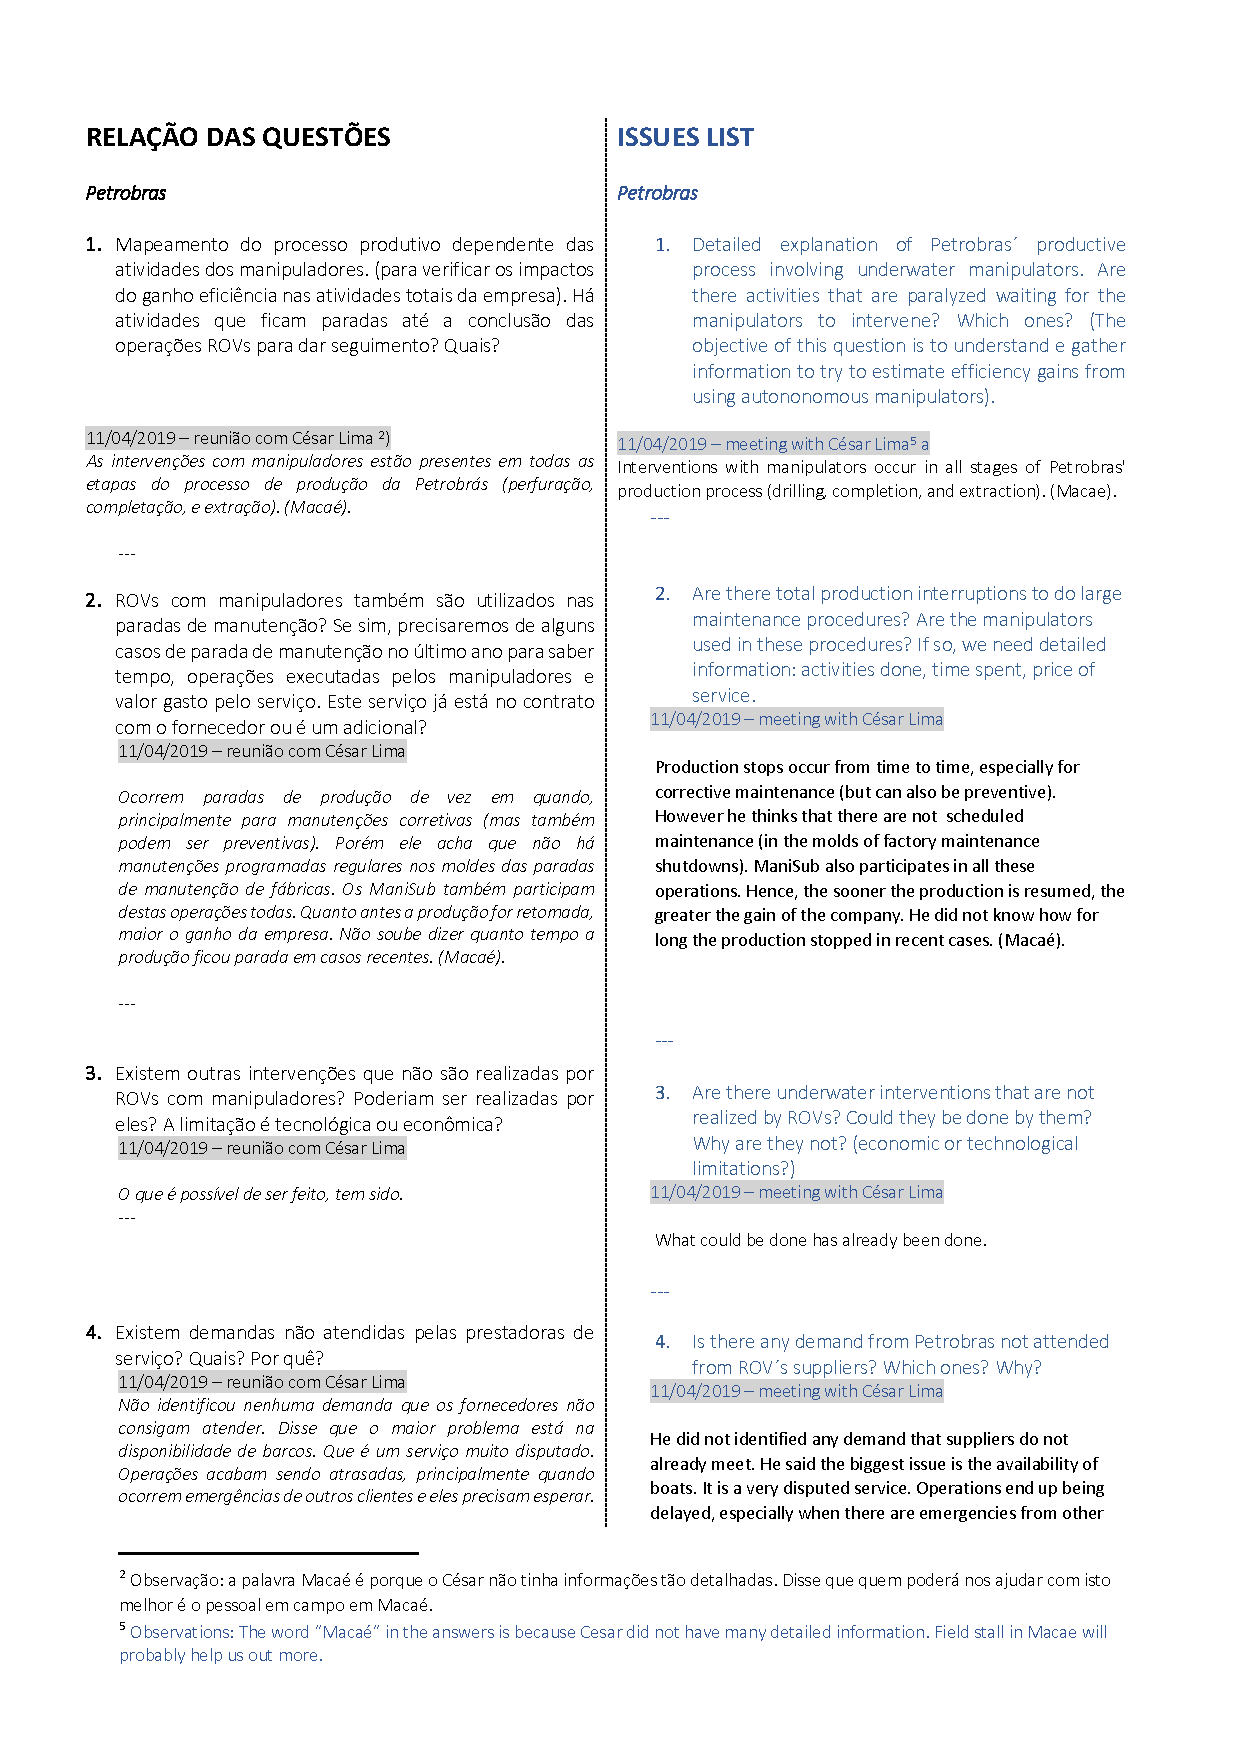
\includepdf[pages={{},-}]{appendix/listquest.pdf}
	% \lipsum[1] % Comentar e adicionar apêndice aqui
	% %
	% \chapter{Um assunto importante}
	% \label{apend:assunto}
	% \lipsum[1] % Comentar e adicionar apêndice aqui
	

% --------------------------------------------------------------------------
% Anexos                                                                     
	% \anexos
	% \justify
	% %
	% \chapter{Outro assunto importante}
	% \label{ann:relant}
	% %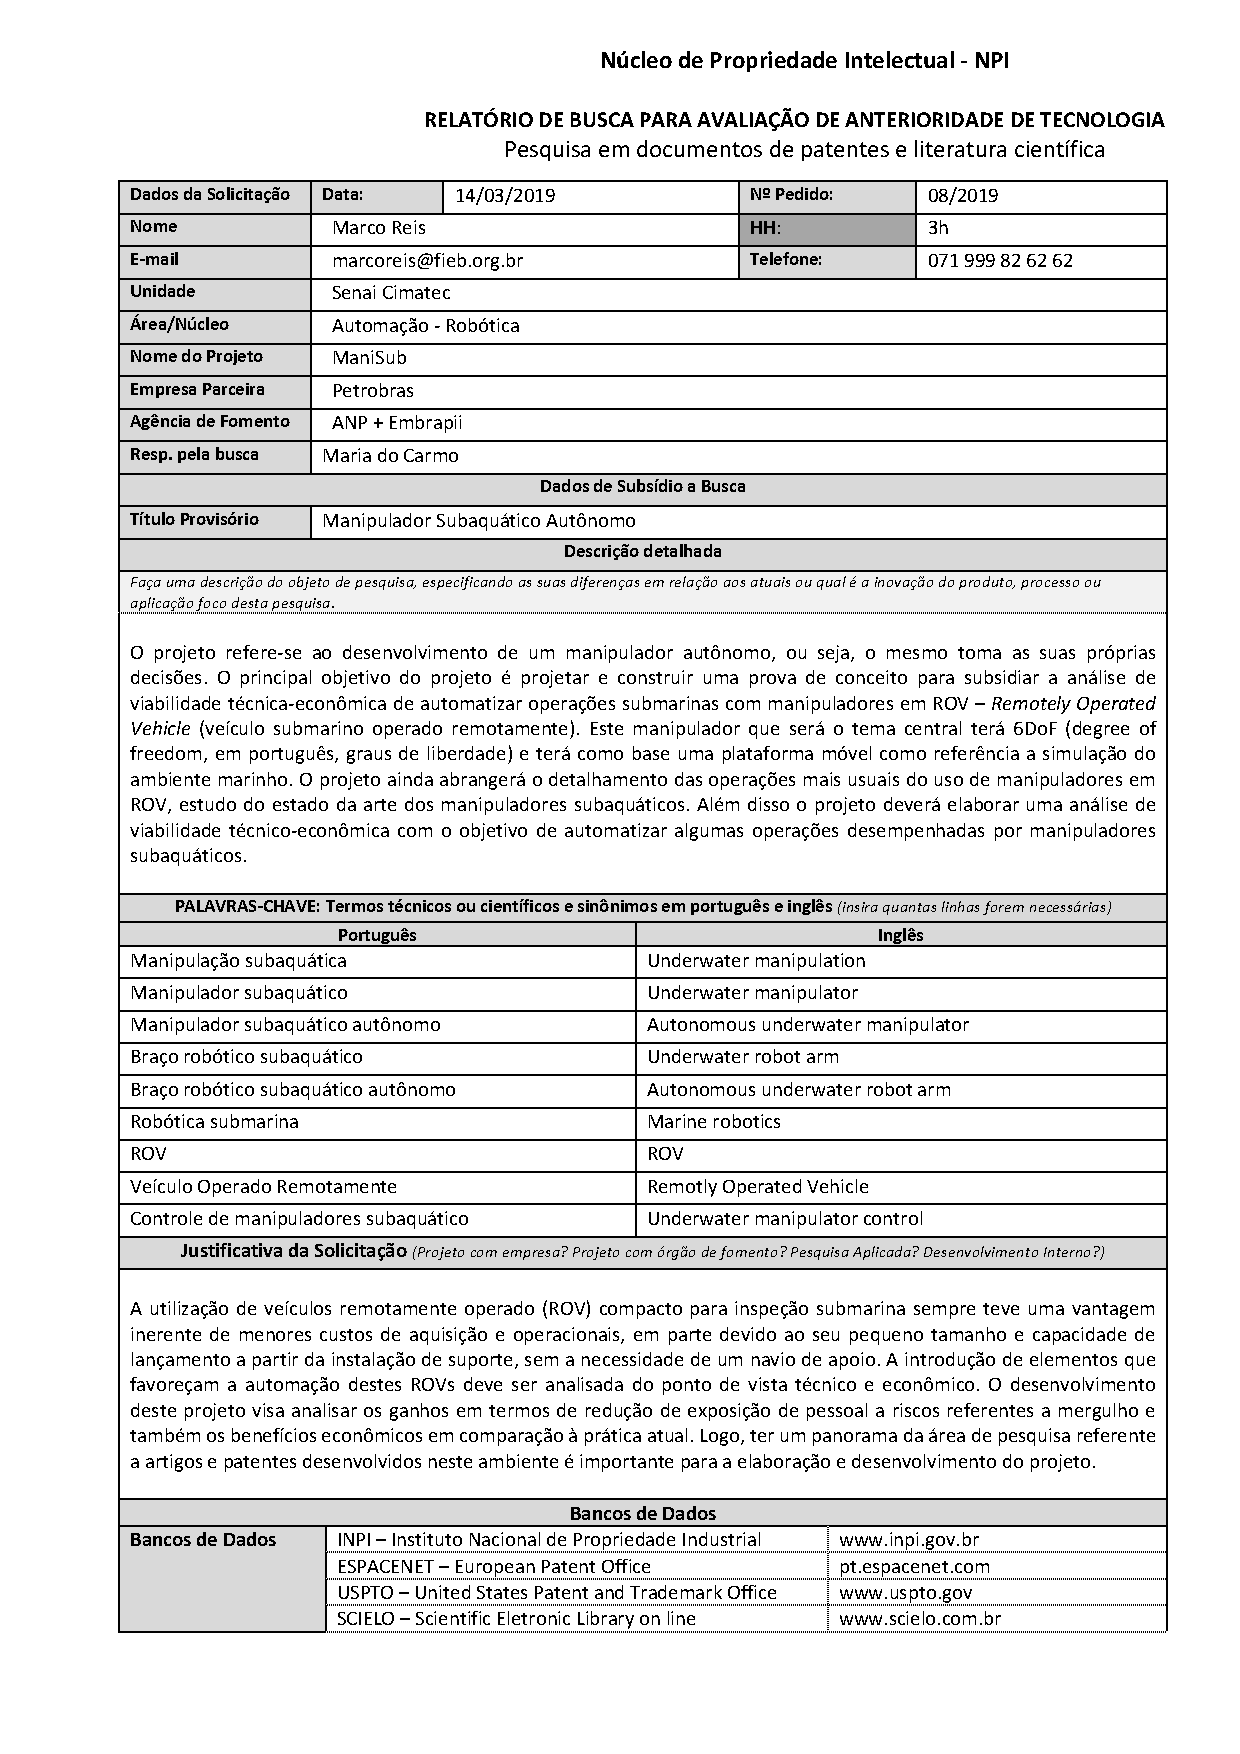
\includepdf[pages={{},-}]{annex/manisubanterioridade.pdf}
	% \lipsum[1] % Comentar e adicionar apêndice aqui
	% %
\end{document} 